% !TeX root = ../courtade-kumar.tex
\begin{figure}[H]
\centering
\definecolor{chainA}{RGB}{140,82,235}
\definecolor{chainB}{RGB}{40,160,235}
\definecolor{chainC}{HTML}{E5A900}
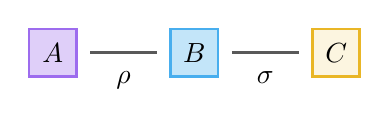
\begin{tikzpicture}[
    bit/.style={minimum width=0.6cm,minimum height=0.6cm,
      inner sep=0pt,outer sep=0pt,line width=1pt},
    edge/.style={line width=1.1pt,draw=black!65,
      shorten <=5pt,shorten >=5pt},
    edge label/.style={midway,below=3pt,inner sep=1pt,
      text height=1.5ex,text depth=0.3ex}]
  \node[bit,draw=chainA!85,fill=chainA,fill opacity=0.28,
    text opacity=1] (A) at (0,0) {$A$};
  \node[bit,draw=chainB!85,fill=chainB,fill opacity=0.28,
    text opacity=1] (B) at (1.8,0) {$B$};
  \node[bit,draw=chainC!85,fill=chainC!12]
    (C) at (3.6,0) {$C$};
  \draw[edge] (A.east) -- node[edge label]
    {$\rho$} (B.west);
  \draw[edge] (B.east) -- node[edge label]
    {$\sigma$} (C.west);
\end{tikzpicture}
\captionsetup{font=small,name=Figure,labelformat=default,labelsep=period,labelfont=bf}
\label{fig:three-bit-chain}
\end{figure}
